\documentclass[12pt]{article}
\usepackage[utf8]{inputenc}
\usepackage[T1]{fontenc}
\usepackage{geometry}
\usepackage{graphicx}
\usepackage{makeidx}
\geometry{margin=2.5cm}
\usepackage{fancyhdr}

\begin{document}
	
	\thispagestyle{empty}
	
	\begin{center}
		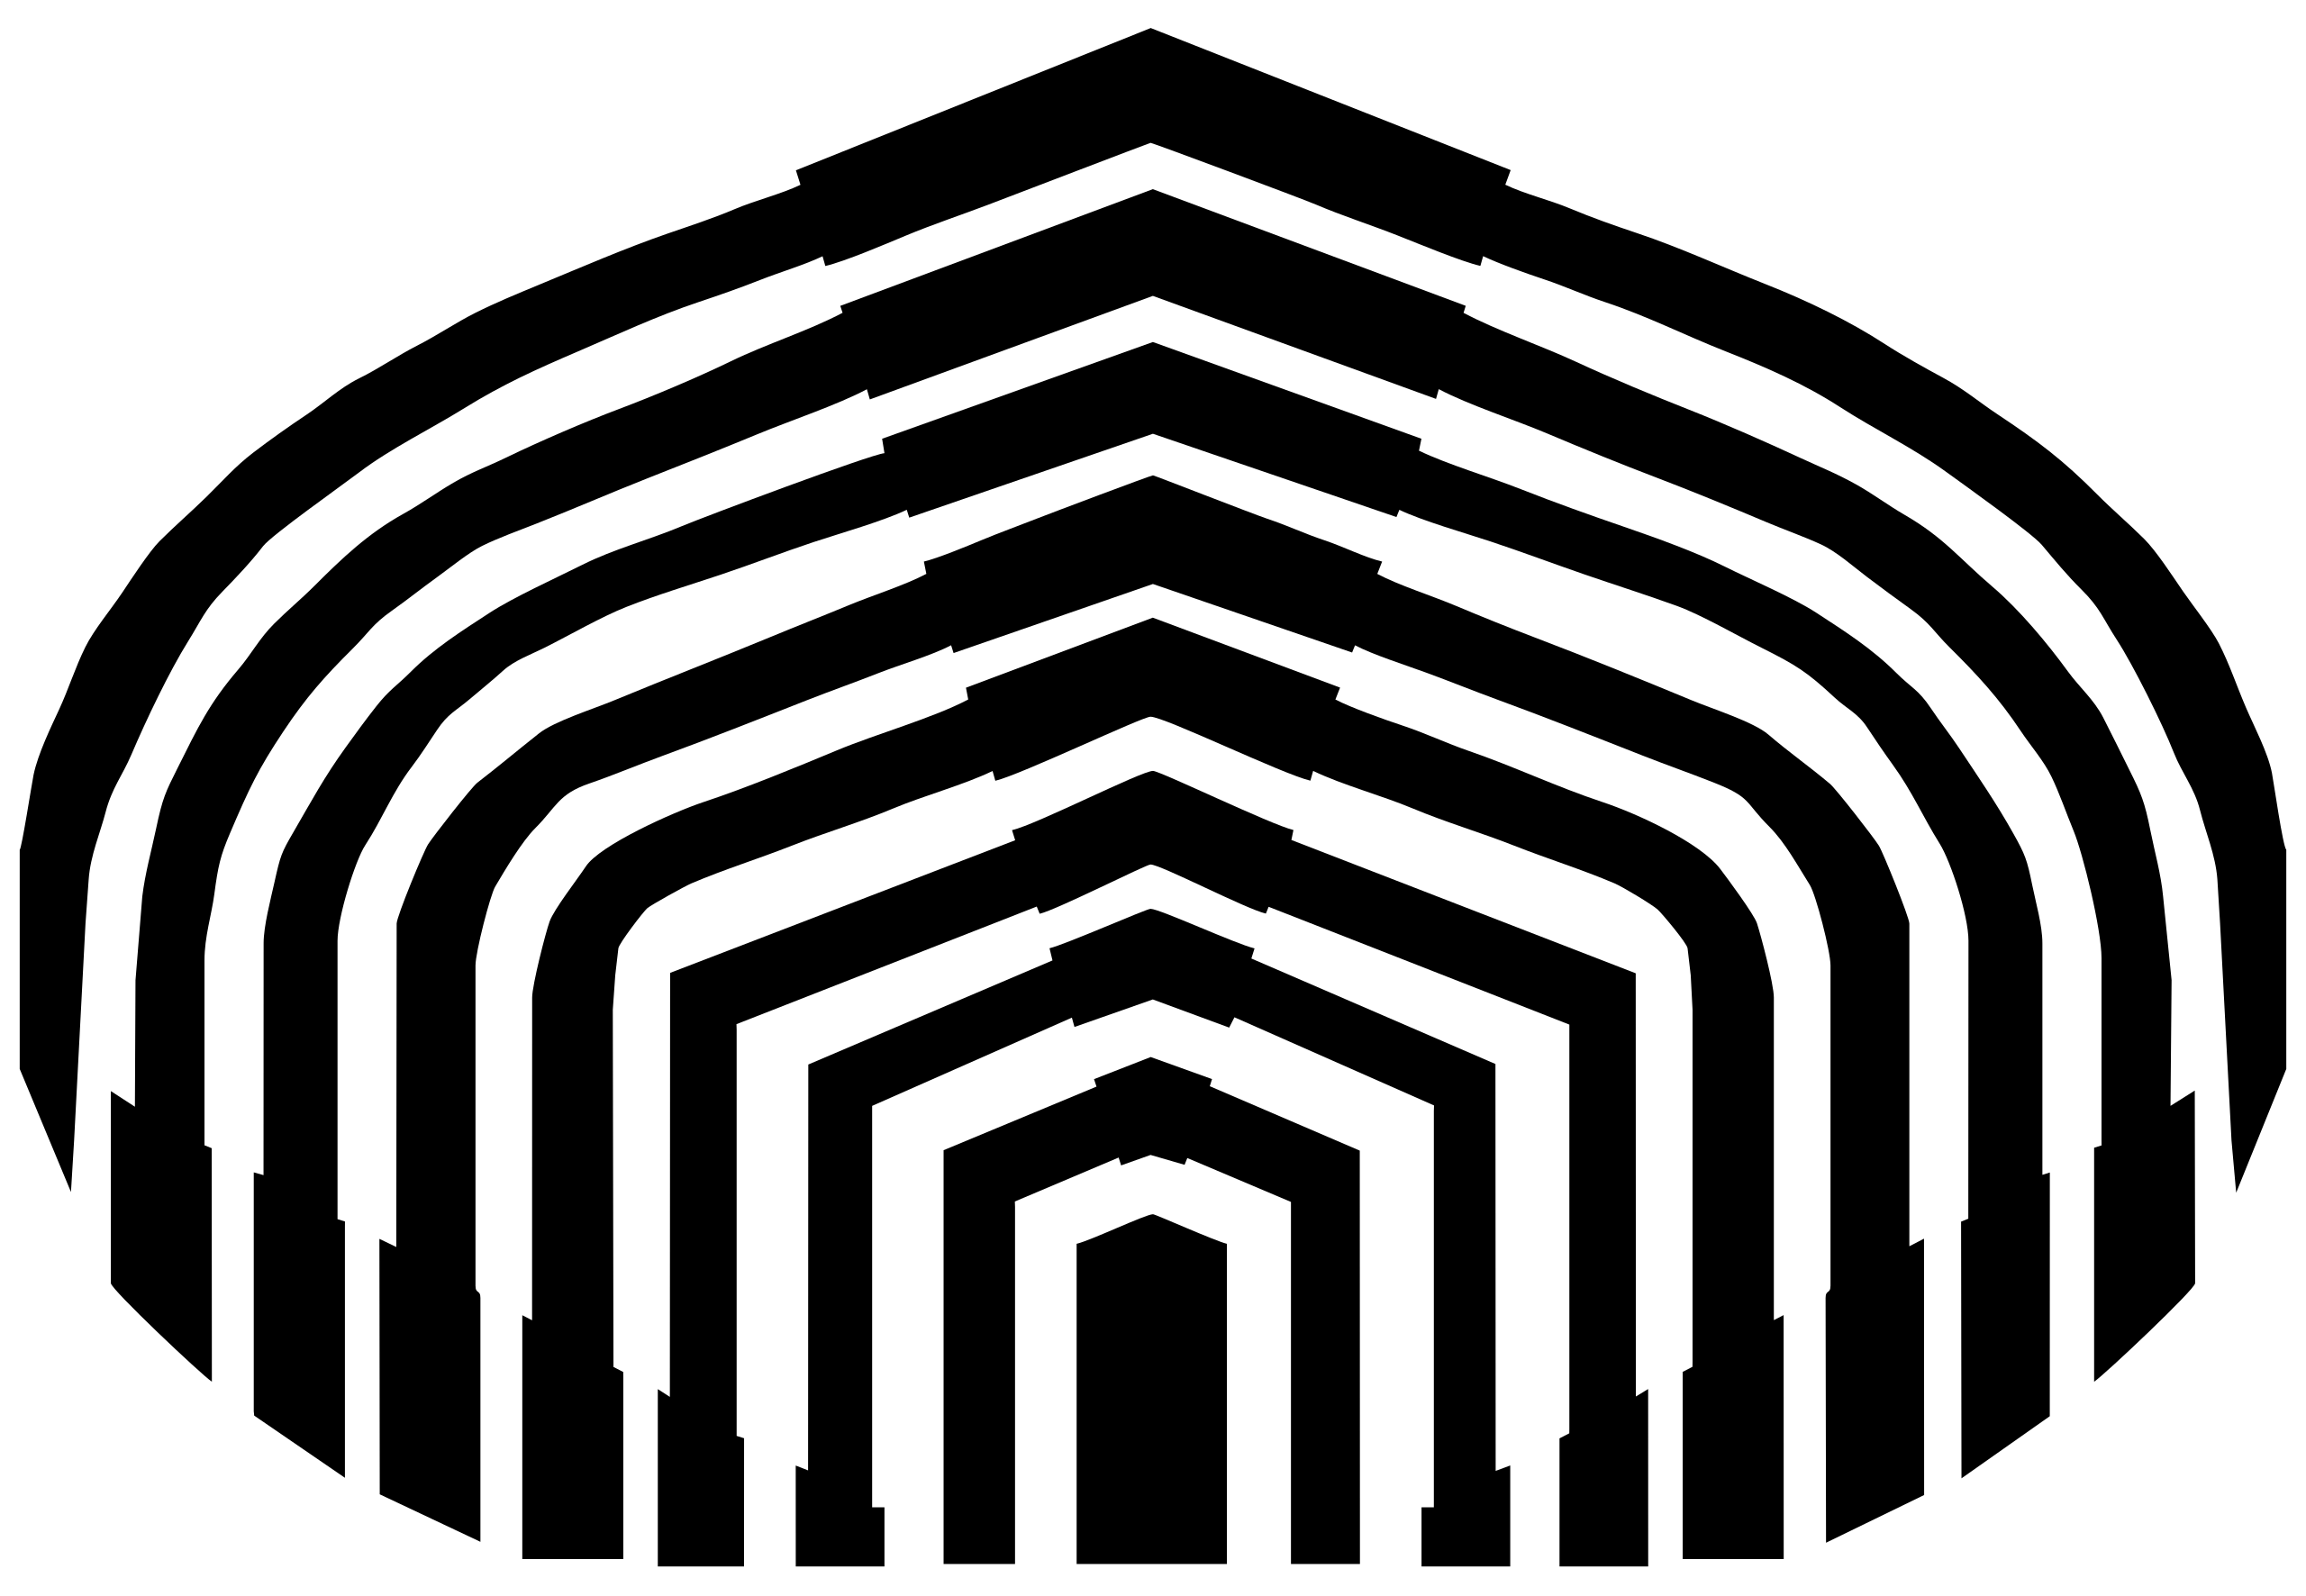
\includegraphics[width=3.1cm,height=2cm]{logo}\\
		UNIVERSIDAD SIMÓN BOLÍVAR\\
		DEPARTAMENTO DE ELECTRÓNICA Y CIRCUITOS\\
		EC1281 - LABORATORIO DE MEDICIONES ELÉCTRICAS\\
		SECCIÓN 1 - GRUPO 1\\
		
		\vspace{7cm}
		\textbf{\Large INFORME - PRÁCTICA \#7}\\
		INSTRUMENTO DE MEDICÓN PARA CORRIENTE ALTERNA (AC)\\
	\end{center}
	
	\begin{flushleft}
		\vspace{9cm}
		\hfill Integrantes:\\
		\hfill {\large Luis Becerra - 1910557}\\
		\hfill {\large Lorena Rojas - 1910469}\\
	\end{flushleft}
	
	\newpage
	
	\pagenumbering{Roman}
        \setcounter{page}{2}
	
	\begin{center}
		\textbf{\large RESUMEN}\\
	\end{center}
	
	En esta práctica de laboratorio, se tuvieron como objetivos principales la interpretación de las características nominales de los instrumentos de medición para corriente alterna (AC) y el uso adecuado de dichos instrumentos en mediciones en AC. Se realizaron mediciones directas e indirectas de voltajes y corrientes pico y rms, mediciones de frecuencia, desfasaje y potencia en circuitos alimentados con fuentes alternas. Además, se compararon los resultados experimentales con los valores teóricos o simulados de los circuitos. Las mediciones se llevaron a cabo utilizando voltímetros, amperímetros, multímetros y osciloscopios. Se realizaron mediciones de resistencias, voltajes pico y rms, corrientes pico, desfasaje y potencia en diferentes configuraciones de circuitos. Los resultados obtenidos fueron analizados y se concluyó sobre la precisión y confiabilidad de los instrumentos de medición utilizados.
	
	\newpage
	
	\begin{center}
		\textbf{\large ÍNDICE}\\
	\end{center}
	
	\noindent \textbf{RESUMEN} \hfill \textbf{II}\\
	\noindent \textbf{ÍNDICE} \hfill \textbf{III}\\
	\noindent \textbf{MARCO TEÓRICO} \hfill \textbf{1}\\
	\noindent \textbf{METEDOLOGÍA} \hfill \textbf{}\\
	\noindent \textbf{RESULTADOS} \hfill \textbf{}\\
	\noindent \textbf{ANÁLISIS DE RESULTADOS} \hfill \textbf{}\\
	\noindent \textbf{CONCLUSIONES} \hfill \textbf{}\\
	\noindent \textbf{BIBLIOGRAFÍA} \hfill \textbf{}\\
	\noindent \textbf{ANEXOS} \hfill \textbf{}\\
	
	\newpage
	
	\pagenumbering{arabic}
	
	\begin{center}
		\textbf{\large MARCO TEÓRICO}\\
	\end{center}
	
	\textbf{1. Valor medio cuadrático (RMS) de una señal alterna}\\
	
	El valor medio cuadrático (RMS, por sus siglas en inglés) es una medida importante para caracterizar una señal alterna. Representa el valor efectivo de la amplitud de una señal y se calcula mediante la raíz cuadrada de la media del cuadrado de los valores instantáneos de la señal a lo largo de un período.\\
	
	Para una señal periódica $V(t)$ con un período $T$, el valor RMS se define como: $$V(t) = \sqrt{\frac{1}{T}*\int_{0}^{T}V^2(t)dt}$$	
	
	Donde $V(t)$ es el valor instantáneo de la señal en un instante de tiempo $t$. El valor RMS es útil porque representa la amplitud equivalente de una señal de corriente alterna en términos de su valor continuo.\\
	
	\textbf{2. Ancho de banda de un circuito o instrumento de corriente alterna}\\
	
	El ancho de banda de un circuito o instrumento de corriente alterna se refiere al rango de frecuencias dentro del cual la respuesta del sistema es aceptablemente buena. Se define como la diferencia entre la frecuencia más alta y la frecuencia más baja que puede ser transmitida o medida por el sistema sin una degradación significativa.\\
	
	En general, el ancho de banda está relacionado con la capacidad del circuito o instrumento para responder a señales de diferentes frecuencias. Los circuitos o instrumentos con un ancho de banda amplio pueden capturar o medir señales de frecuencia más alta, mientras que aquellos con un ancho de banda más estrecho tienen una respuesta limitada a frecuencias altas.\\
	
	El ancho de banda puede estar determinado por la capacidad de los componentes del circuito, como condensadores e inductores, así como por la respuesta de los amplificadores o filtros utilizados en el sistema. Es importante considerar el ancho de banda al seleccionar un circuito o instrumento de corriente alterna para asegurarse de que pueda manejar las frecuencias de interés.\\
	
	\textbf{3. Instrumentos de medición de voltajes y corrientes AC}\\
	
	Existen varios tipos de instrumentos de medición utilizados para medir voltajes y corrientes en circuitos de corriente alterna (AC). Estos instrumentos ofrecen diferentes características y se utilizan en diferentes aplicaciones según las necesidades del usuario.
	
	\begin{itemize}
		\item \textbf{Voltímetro de AC:} Este instrumento se utiliza para medir el valor eficaz o RMS de un voltaje AC. Puede tener escalas y rangos variables para adaptarse a diferentes niveles de voltaje. Algunos voltímetros de CA también pueden medir frecuencia y desfasaje.
		
		\item \textbf{Amperímetro de AC:} Este instrumento se utiliza para medir el valor eficaz o RMS de una corriente AC. Al igual que el voltímetro de CA, puede tener escalas y rangos variables para adaptarse a diferentes niveles de corriente. Algunos amperímetros de CA también pueden medir frecuencia y desfasaje.
		
		\item \textbf{Multímetro:} Es un instrumento versátil que combina funciones de voltímetro, amperímetro y ohmímetro. Puede medir voltajes y corrientes AC en diferentes rangos, así como resistencias y otras magnitudes eléctricas. Algunos multímetros también tienen capacidades de medición de frecuencia y desfasaje.
		
		\item \textbf{Osciloscopio:} Es un instrumento utilizado para visualizar y analizar formas de onda de señales eléctricas. Puede mostrar la amplitud, frecuencia, forma de onda y desfasaje de una señal AC en una pantalla. Los osciloscopios también pueden realizar mediciones precisas de voltajes y tiempos en señales AC.
		
	\end{itemize}
	
	Cada tipo de instrumento tiene sus ventajas y limitaciones, y la elección depende del tipo de medición requerida, el rango de frecuencias de interés y la precisión necesaria.

	\newpage
	
	\begin{center}
		\textbf{\large METODOLOGÍA}\\
	\end{center}
	
	\renewcommand{\theenumi}{\alph{enumi}} %Letras minúsculas 
	
	\begin{enumerate}
		
		\item Determinación experimental del equivalente Thevenin:\\
		
		Tal y como se estudió en EC1251, el teorema de Thevenin es una simplificación que podemos aplicar para circuitos con elementos lineales, donde se reduce el circuito a un voltaje de Thevenin y una resistencia de Thevenin entre dos puntos $A$ y $B$. El equivalente de Thevenin de un circuito permite facilitar la operación del mismo respecto a un par de nodos de interés, haciendo mucho más simples los cálculos y manipulación del mismo. El circuito al cual se le determinó el equivalente de Thevenin fue:
		
		\begin{center}
			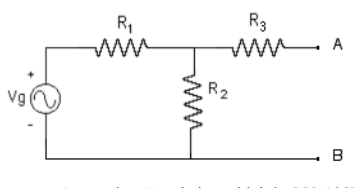
\includegraphics[width=16cm,height=8cm]{Img/circ_1}
		\end{center}
		
		Los valores nominales utilizados para este circuito fueron $V_g = 5V$, $f = 100Hz$, $R_1 = R_2 = 2k\Omega$ y $R_3 = 1k\Omega$.\\
		
		A partir de esos valores y esa configuración de circuito se procedió a realizar algunas medidas para calcular el equivalente de Thevenin. Se midió el voltaje de Thevenin mediante el osciloscopio y un voltímetro, también se midió la corriente de Norton con un amperímetro y con el osciloscopio usando una resistencia de $51,3\Omega$. Con el osciloscopio se obtuvieron los valores pico. A partir de eo datos se desarrolló se obtuvo el valor de Thevenin para las resistencias.\\
		
		\item Teorema de Máxima transferencia de Potencia:\\
		
		El teorema de máxima transferencia de potencia establece que, dada una fuente, con una resistencia de fuente fijada, la resistencia de carga que maximiza la transferencia de potencia es aquella con un valor óhmico igual a la resistencia de fuente.\\
		
		De allí se obtiene la idea de cómo variar la resistencia para obtener la máxima potencia, en los experimentos se realizan dos configuraciones, la primera variando la resistencia de Thevenin y la segunda variando la resistencia $R_L$.
		
		\begin{center}
			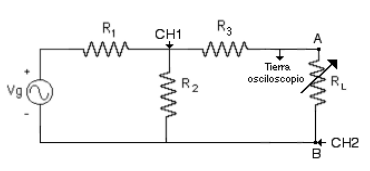
\includegraphics[width=16cm,height=8cm]{Img/circ_2}
		\end{center}
		
		\begin{center}
			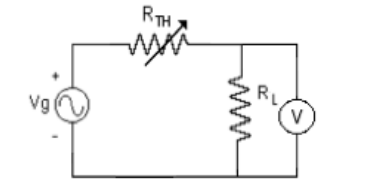
\includegraphics[width=16cm,height=8cm]{Img/circ_3}
		\end{center}
		
		A partir de allí se usaron las mismas resistencias y $V_g$ que antes, en el caso en el que se varía la resistencia de Thevenin se usó una resistencia de $2k\Omega$.
		
		\item Impedancias en un circuito:\\
		
		Para este experimento se usó un circuito al cual se le tomaron mediciones en distintos puntos, los cuales fueron:\\
		
		\begin{center}
			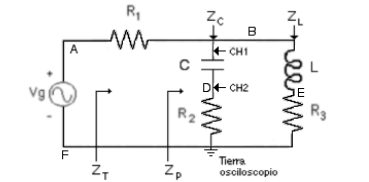
\includegraphics[width=16cm,height=8cm]{Img/circ_4}
		\end{center}
		
		\begin{center}
			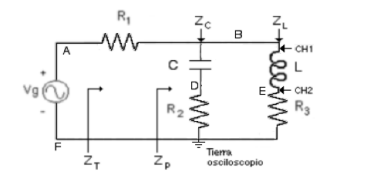
\includegraphics[width=16cm,height=8cm]{Img/circ_5}
		\end{center}
		
		\begin{center}
			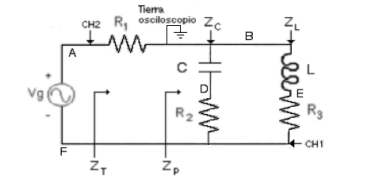
\includegraphics[width=16cm,height=8cm]{Img/circ_6}
		\end{center}
		
		Y a partir de allí se determinaron las impedancias y el defase partiendo de tres resistencias cuyo valor nominal era $1k\Omega$, un condensador de $100nF$, un inductor de $100mH$ y una fuente de $10V$ pico a $1kHz$. Luego siguiendo leyes circuitales se determinó la impedancia.
		
		\item Operación de un medidor de verdadero valor rms y un vatímetro digital:\\
		
		Para este experimento se usó un variac, un dimmer, un bombillo y los distintos aparatos de medición. Lo que se hizo fue que primero se variaba el voltaje con el variac para modificar el la potencia disipada en el bombillo y tomar las medidas en los distintos instrumentos, luego, se realizó el mismo proceso con el dimmer, un aparato para regular la potencia disipada sin disminuir el voltaje.
		
		
	\end{enumerate}
	
	\newpage
	
	\begin{center}
		\textbf{\large RESULTADOS}\\
	\end{center}
	
	A continuación se presentan los resultados obtenidos durante el trabajo en el laboratorio:
	
	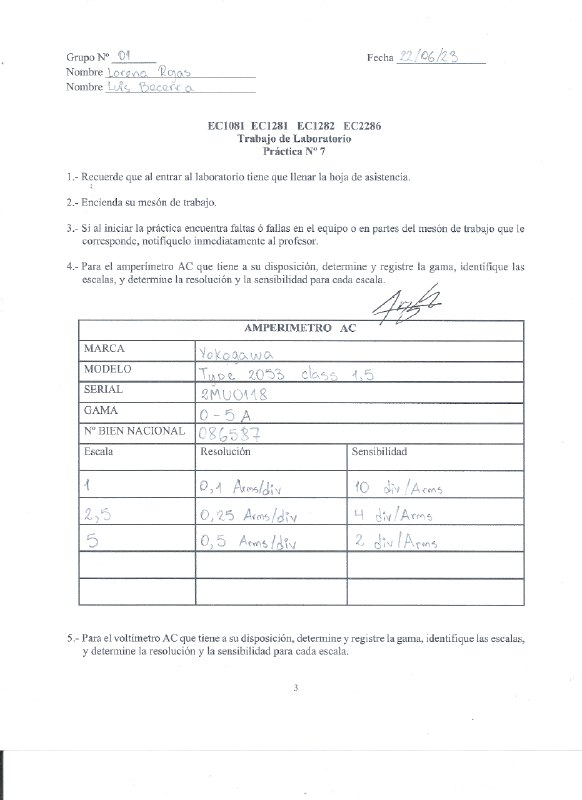
\includegraphics[width=16cm,height=21cm]{Img/Resultados_1}\\
	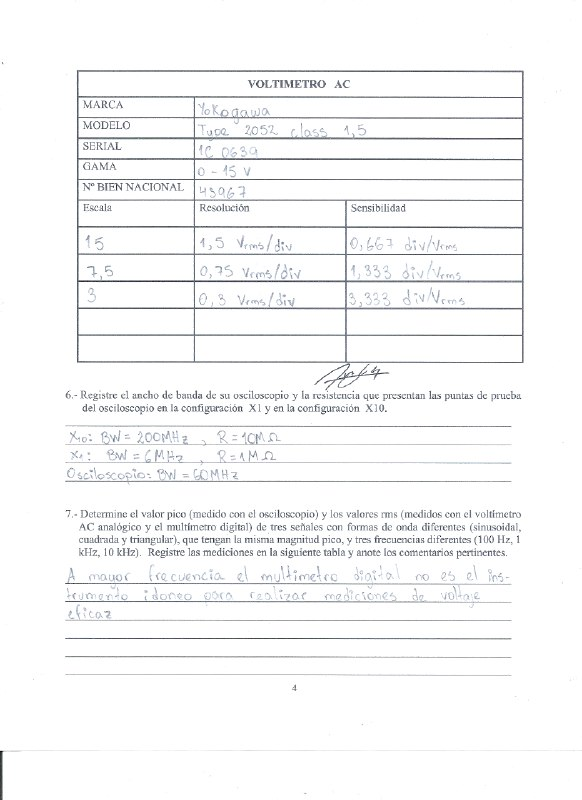
\includegraphics[width=16cm,height=21cm]{Img/Resultados_2}\\
	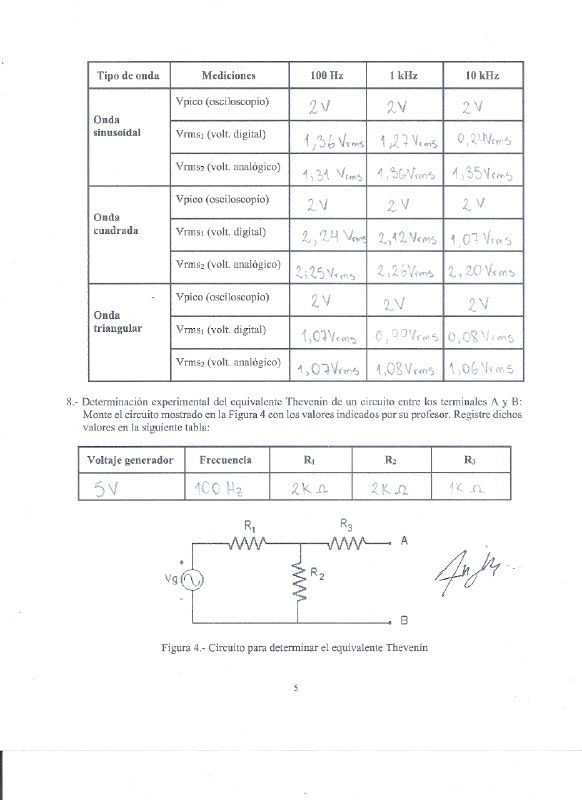
\includegraphics[width=16cm,height=21cm]{Img/Resultados_3}\\
	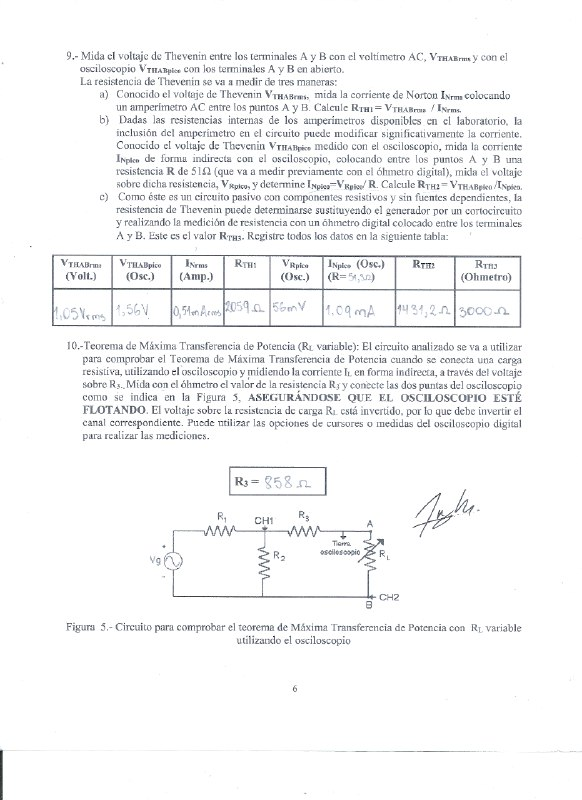
\includegraphics[width=16cm,height=21cm]{Img/Resultados_4}\\
	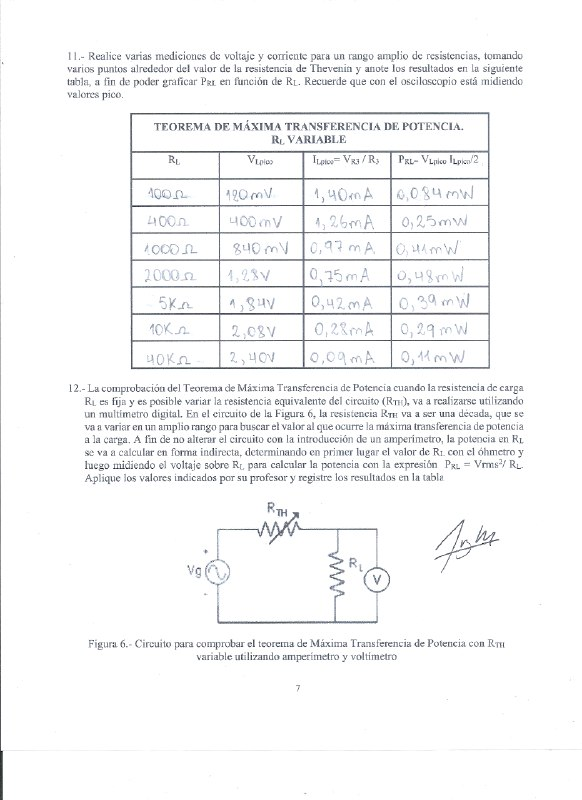
\includegraphics[width=16cm,height=21cm]{Img/Resultados_5}\\
	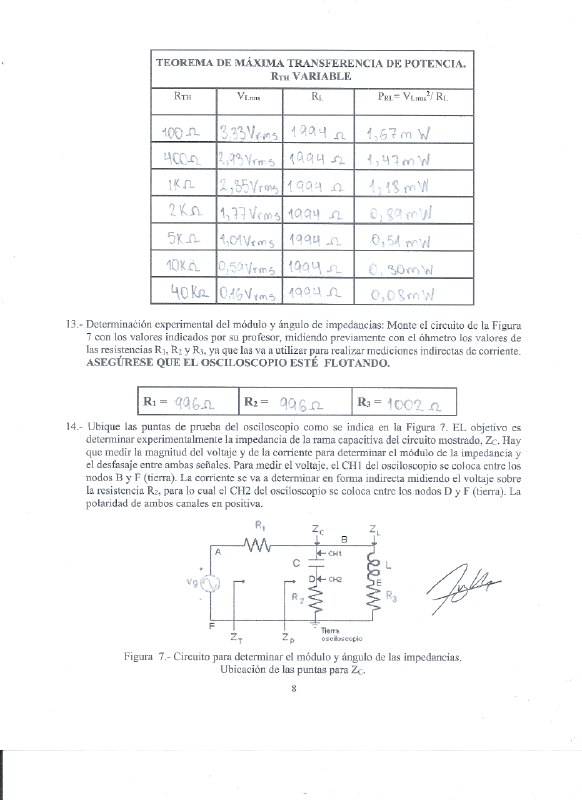
\includegraphics[width=16cm,height=21cm]{Img/Resultados_6}\\
	
	\noindent 15.- Ubicadas las puntas de prueba según lo indicado, realice la medición del voltaje pico en la rama $Z_{C}$, el voltaje pico sobre la resistencia $R_{2}$ para calcular la corriente pico en dicha rama y el desfasaje entre ambas señales, el cual es el ángulo de la impedancia $Z_{C}$. Calcule el módulo de dicha impedancia ($V/I$) y registre todos los valores en las casillas correspondientes. Tome una foto de las señales observadas.
	
	\begin{center}
		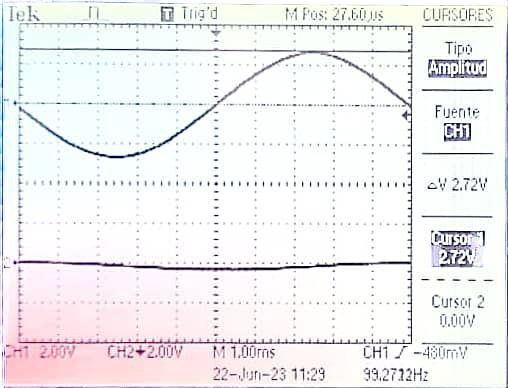
\includegraphics[width=10cm,height=6cm]{Img/resul_15}\\
	\end{center}
	
	\noindent 16.- Para determinar experimentalmente la impedancia de la rama inductiva ZL coloque ahora la punta del CH1 en el nodo B y la del CH2 en el nodo E, con la tierra en el nodo F, como se indica en la Figura 8. Realice las mediciones del voltaje pico en la rama, el voltaje pico sobre la resistencia R3 para calcular la corriente pico por la rama, y el desfasaje entre ambas señales. Calcule el módulo de la impedancia para este caso, registre los datos en las casillas disponibles y tome una foto de las señales observadas.
	
	\begin{center}
		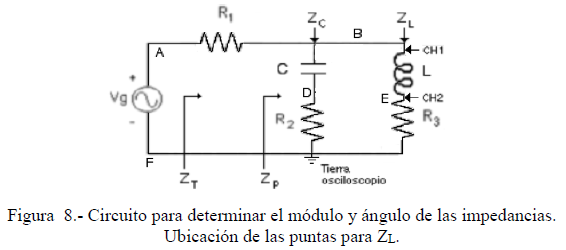
\includegraphics[width=10cm,height=5cm]{Img/Captura}\\
		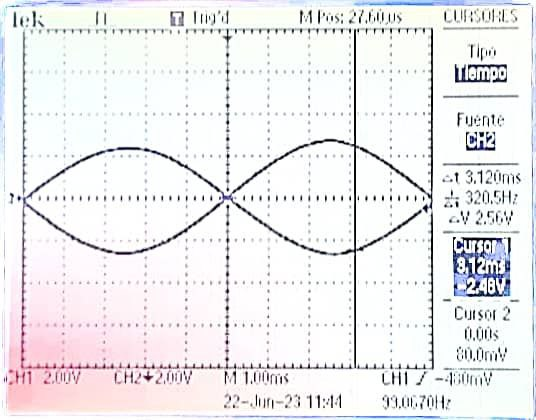
\includegraphics[width=10cm,height=6cm]{Img/resul_16}\\
	\end{center}
	
	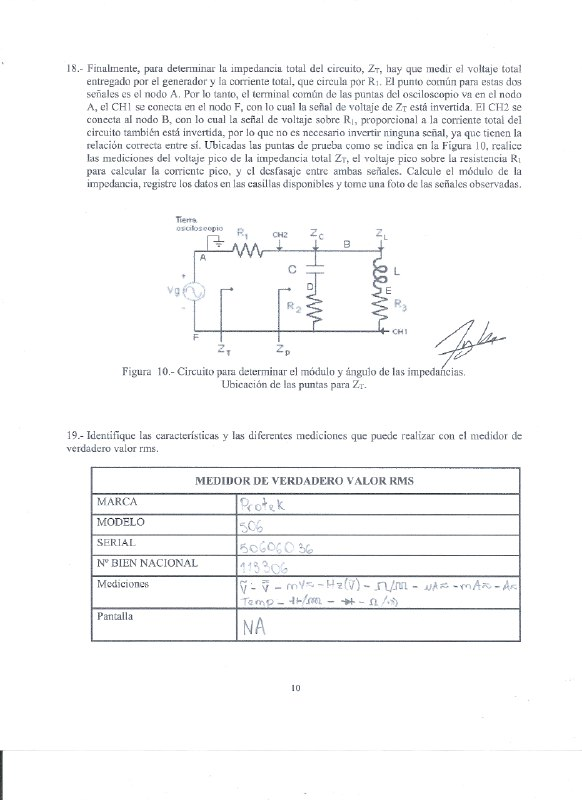
\includegraphics[width=16cm,height=21cm]{Img/Resultados_7}\\
	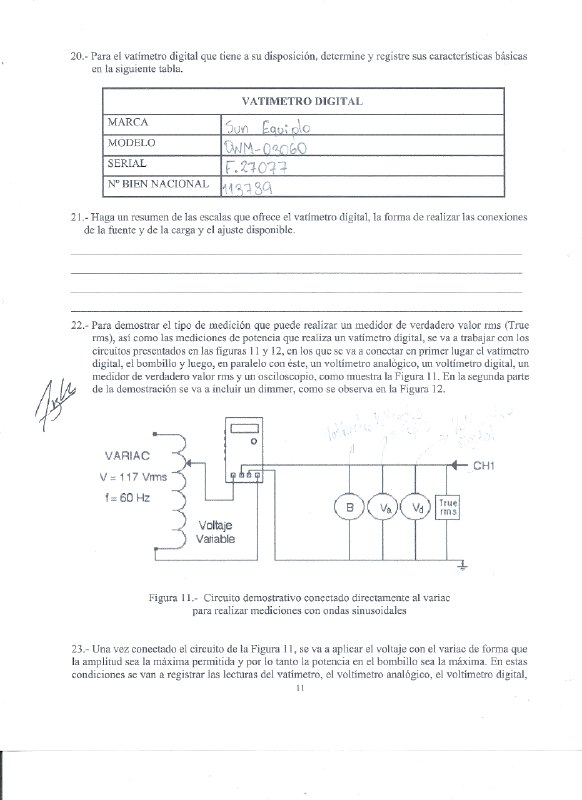
\includegraphics[width=16cm,height=21cm]{Img/Resultados_8}\\
	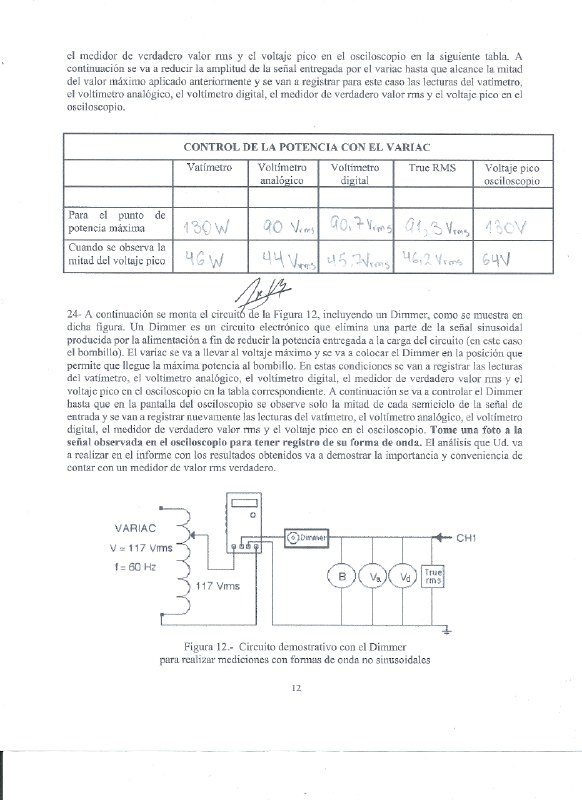
\includegraphics[width=16cm,height=21cm]{Img/Resultados_9}\\
	
	\begin{center}
		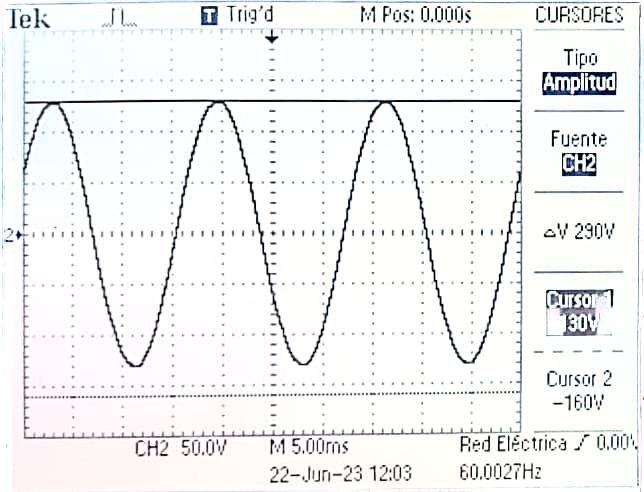
\includegraphics[width=12cm,height=8cm]{Img/resul_22_1}\\
		\textit{Potencia Máxima}\\
		\vspace{2cm}
		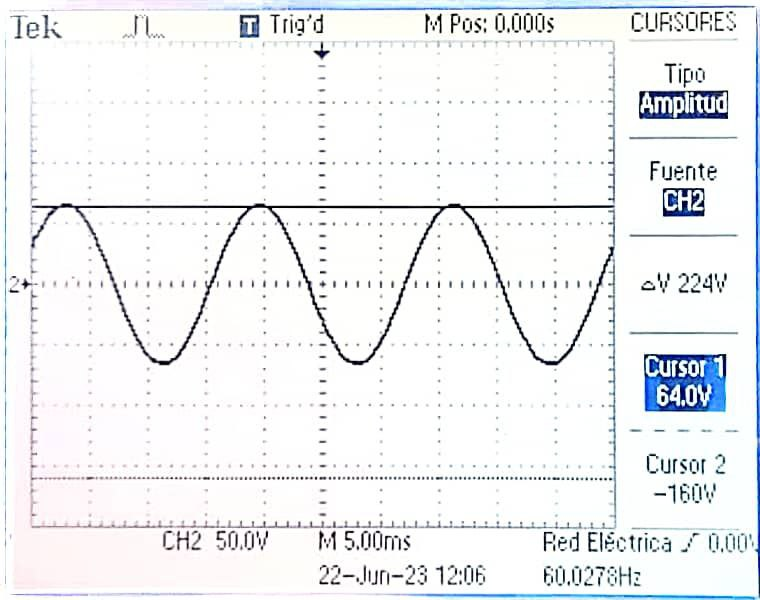
\includegraphics[width=12cm,height=8cm]{Img/resul_22_2}\\
		\textit{A la mitad del voltaje pico}
	\end{center}

	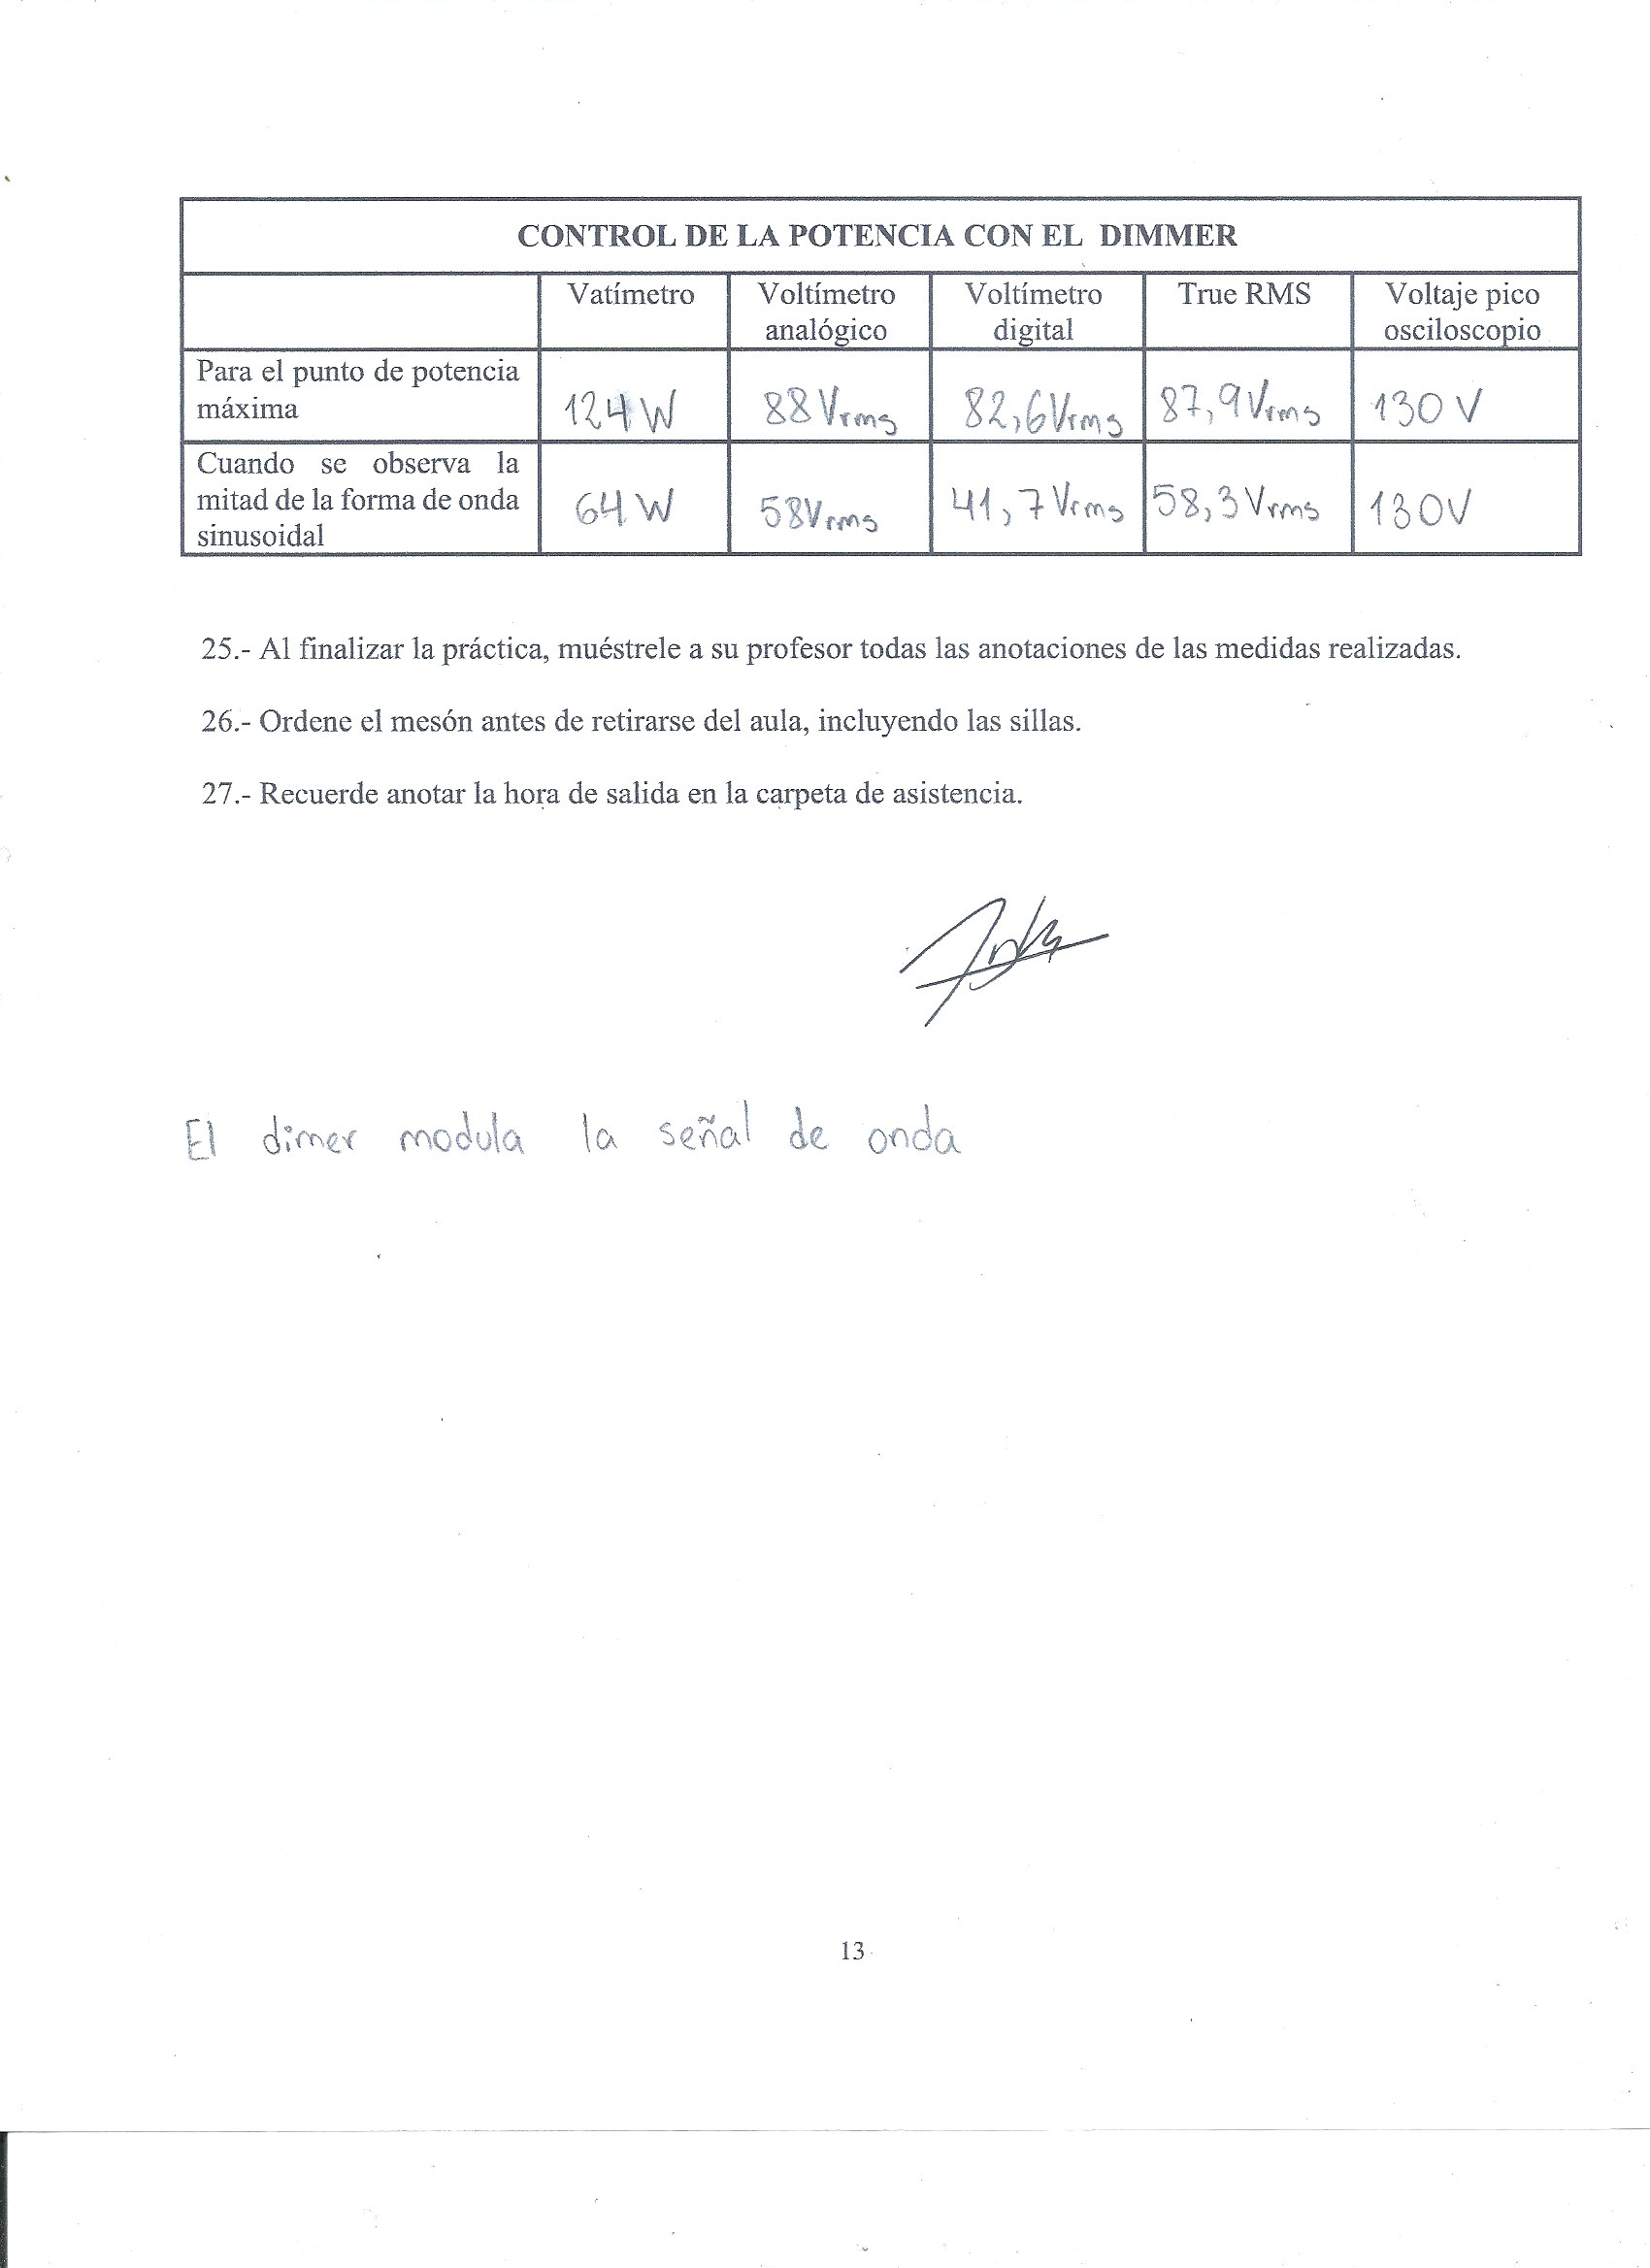
\includegraphics[width=16cm,height=21cm]{Img/Resultados_10}\\
	
	\begin{center}
		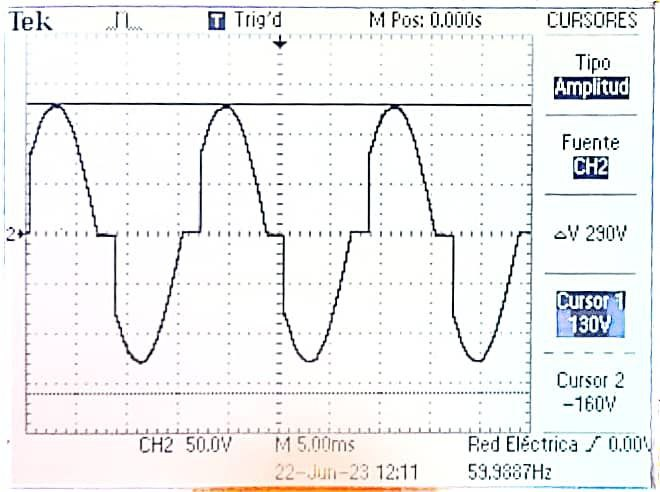
\includegraphics[width=12cm,height=8cm]{Img/resul_24_1}\\
		\textit{Potencia Máxima}\\
		\vspace{2cm}
		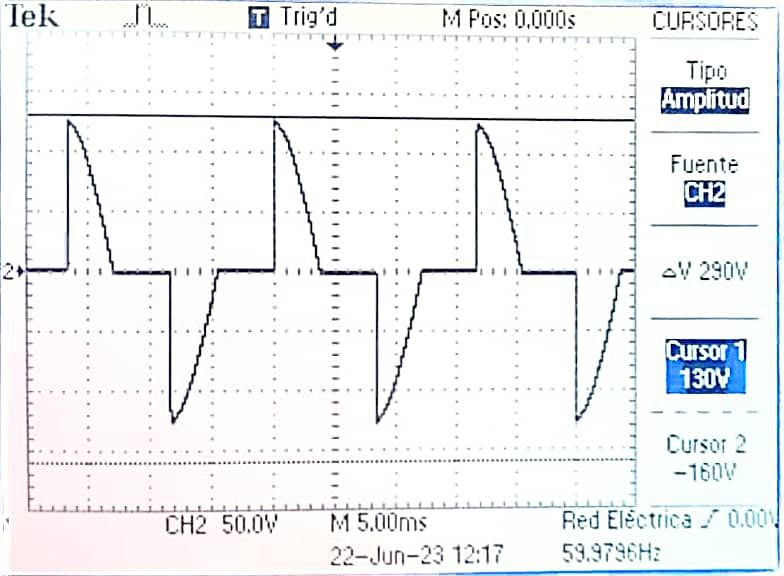
\includegraphics[width=12cm,height=8cm]{Img/resul_24_2}\\
		\textit{A la mitad de la forma de la onda sinusoidal}\\
	\end{center}
	
	\newpage
	
	\begin{center}
		\textbf{\large ANÁLISIS DE RESULTADOS}\\
	\end{center}
	
	\renewcommand{\theenumi}{\alph{enumi}} %Letras minúsculas 
	
	\begin{enumerate}
		
		\item Mediciones del valor pico y el valor
		rms para las tres señales periódicas a diferentes frecuencias:
		
		\noindent Es conocido que los voltímetros con los que se realizó la práctica miden el valor rms de ondas sinusoidales en ciertas frecuencias, es decir, su algorítmo está adaptado para el cálculo de ese tipo de onda basados en la operación $\frac{A}{\sqrt{2}}$.\\
		
		\noindent Se pudo evidenciar durante las mediciones que al cambiar el tipo de onda o la frecuencia de la onda, los voltímetros medían valores cada vez menos exactos. El voltímetro menos exacto fue el digital, que ya para frecuencias de $1kHz$ arrojaba valores inexactos y ya para los $10kHz$ arrojaba un valor sin sentido.\\
		
		\noindent Ambos voltímetros arrojaban un valor rms mayor para ondas cuadradas y menos para ondas triagulares. Estos instrumentos pueden ser utilizados para dichas mediciones pero ya es conocido que no sería óptimo y que pueden traer consigo errores sustanciales.
		
		\item Valores obtenidos para la resistencia de Thevenin:
		
		\noindent Para la resistencia de Thevenin se obtuvieron tres medidas, de las cuales la más cercana fue la primera, donde se midió la corriente de Norton mediante un amperímetro y el voltaje de Thevenin mediante un voltímetro, esto resultó en un valor de $2059\Omega$, que fue el más cercano a los $2000\Omega$ que se tenían mediante valores nominales. Los otros valores medidos tuvieron errores notables debido a resistencias internas y cómo estas interactuaban con el circuito, midiendo la corriente de Norton y voltaje de Thevenin el error se redujo al mínimo.
		
		\item Gráficas de $P_{RL}$ y $R_L$:
		
		\begin{center}
			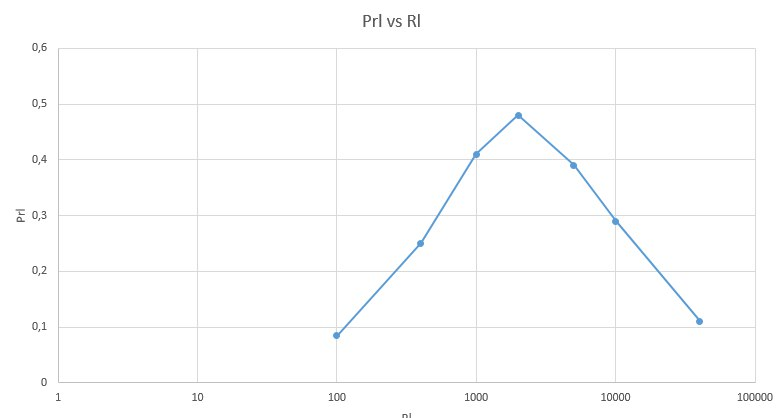
\includegraphics[width=16cm,height=8cm]{Img/graph_1}
		\end{center}
	
		\begin{center}
			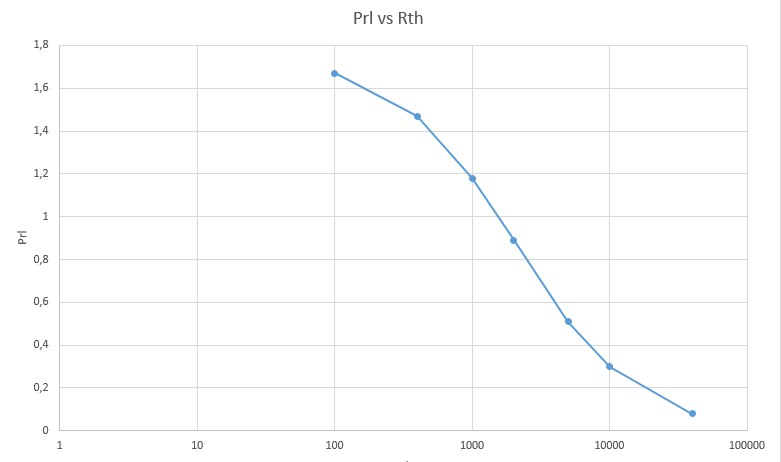
\includegraphics[width=16cm,height=8cm]{Img/graph_2}
		\end{center}\\
	
		\noindent Es conocido que la máxima transferencia de potencia se da cuando la resistencia de la carga es equivalente a la resistencia de Thevenin, en el primer experimento se varía la carga $R_L$. La potencia máxima se alcanza cuando $R_L$ alcanza el valor de resistencia de $R_{TH}$, es decir, alrededor de $2k\Omega$.\\
		
		\noindent En el segundo experimento se varía $R_{TH}$ y se deja $R_L$ fijo, cabe a destacar que para este experimento se conecta un voltímetro a $R_L$ el cual tiene una resistencia interna que influye en el sistema. En este caso $R_{TH}$ está en serie con el paralelo de $R_L$ y la resistencia interna del voltímetro, lo cual modifica su valor, dando como resultado que la máxima transferencia de potencia esté en $R_{TH} = 100\Omega$.
		
		\item Los valores de las impedancias:
		
		\noindent En la teoría se conoce que en circuitos AC, la impedancia resistiva tiene $0^{\circ}$ de defase, la inductiva $90^{\circ}$ donde el voltaje adelanta a la corriente y la capacitiva $90^{\circ}$ donde la corriente adelanta al voltaje. Para las medidas tomadas se obtuvo $Z_C = 1,6k\angle96,5^{\circ}\Omega$, $Z_L = 1133,33\angle 91,30^{\circ}\Omega$, $Z_p = 1026,81\angle 0^\circ \Omega$ y $Z_T = 432,95\angle 0^\circ \Omega$, lo cual se corresponde perfectamente con lo planteado en la teoría.
		
		\item Medición de los distintos instrumentos:
		
		\noindent Al estudiar la potencia disipada por un bombillo, se montaron dos circuitos a los cuales se conectaron distintos instrumentos de medición.\\
		
		\noindent Primero se conectó el circuito al variac para disminuir la potencia consumida al disminuir el voltaje, se vislumbró que esta manera es poco práctica ya que es difícil adquirir tal tecnología en casa para el uso diario. Por otro lado, se puede notar que en ambos consumos de potencia todos los voltímetros dan valores bastante exactos en su medición.\\
		
		\noindent Para el segundo circuito, en lugar de usar el variac, se usó un dimmer, un dispositivo electrónico que permite regular el consumo de potencia sin variar el voltaje. Es acá donde surgieron problemas en los voltímetros ya que para el máximo consumo de potencia que se configuró, las mediciones eran adecuadas, mientra que al disminuir la potencia consumida mediante el dimmer, pese a que el voltaje seguía igual, la lectura de los voltímetros cayó como si se estuviera alterando el voltaje, esto debido al funcionamiento de estos dispositivos.
		
	\end{enumerate}
	
	\newpage
	
	\begin{center}
		\textbf{\large CONCLUSIONES}\\
	\end{center}
	
	Inserte conclusiones
	
	\newpage
	
	\begin{center}
		\textbf{\large BIBLIOGRAFÍA}\\
	\end{center}
	
	Inserte bibliografía
	
	\newpage
	
	\begin{center}
		\textbf{\large ANEXOS}\\
	\end{center}
	
	Inserte anexos
	
\end{document}
